\begin{thmBox}{Alternative Definition of Connectedness}[thm:23.1]
    A space \( X \) is connected if and only if the only subsets of \( X \) that
    are both open and closed in \( X \) are the empty set and \( X \) itself.

    \baseSkip

    Said slightly differently, we say that a space \( X \) is connected if and 
    only if it contains no non-trivial clopen subsets.

    \baseRule

    \begin{proofBox}*
        \wrapBox{\( \implies \)}

        Let's say that \( X \) is connected.
        Towards a contradiction, we assume that there exists a nonempty 
        proper subset \( A \) of \( X \) such that it is both open and closed in \( X \).
        We can see that \( U = A \) and \( V = X \setminus A \) constitute
        a separation of \( X \), for they are open, disjoint, nonempty,
        and their union is in \( X \).
        By definition, we have that \( X \) is not connected, which is a 
        contradiction.
        Hence, the only subsets of \( X \) that
        are both open and closed in \( X \) are the empty set and \( X \) itself.

        \baseSkip 

        \wrapBox{\( \impliedby \)}

        Let's now assume that the only subsets of \( X \) that
        are both open and closed in \( X \) are the empty set and \( X \) itself.
        Towards a contradiction, we assume that \( X \) is not connected.
        It follows by definition that there exists a separation of \( X \).
        If \( U \) and \( V \) form this separation of \( X \), then we see that
        \( U \) must be nonempty and different from \( X \) (if it were \( X \),
        then we would have \( V \) to be the \( \emptyset \)), and we have that 
        \( U \) is both open and closed in \( X \) since both \( U \) and \( X 
        \setminus U = V \) are open by definition.
        This gives us a contradiction, which tells us that \( X \) is 
        connected.
    \end{proofBox}
\end{thmBox}

\begin{thmBox}[Lemma]{23.1}[lem:23.1]
    If \( Y \) is a subspace of \( X \), a separation of \( Y \) is a pair of 
    disjoint nonempty sets \( A \) and \( B \) whose union is \( Y \),
    neither of which contains a limit point of the other.
    The space \( Y \) is connected if there exists no separation of \( Y \).

    \baseRule

    \begin{proofBox}
        We essentially want to show that the following are equivalent: 
        \begin{enumerate}
            \item a pair of disjoint nonempty sets \( A \) and \( B \) of 
                \( X \) whose union is \( Y \) and neither of which contains
                a limit point of the other
            \item a pair of disjoint nonempty open sets \( A \) and \( B \)     
                in \( Y \) whose union (in \( Y \)) is \( Y \); that is, 
                \( A \) and \( B \) are both open and closed in \( Y \).
        \end{enumerate}
        We start by showing that \( ( 1 ) \implies ( 2 ) \).
        It suffices to show that both \( A \) and \( B \) are closed in \( Y \);
        this is because if \( A \) is closed in \( Y \), then 
        \( Y \setminus A = B \) is open in \( Y \), and the same can be said
        to show that \( A \) is open in \( Y \) using the fact that \( B \) is 
        also closed in \( Y \).

        \baseSkip

        WLOG, we shall show that \( A \) is closed in \( Y \).
        We start by noting that \( \overline{ A } \) (the closure of \( A \) in
        \( X \)) is closed in \( X \).
        Thus, we have by definition, that \( Y \cap \overline{ A } \) is closed
        in \( Y \).
        If we define \( A' \) to be the set of limit points of \( A \) in 
        \( X \), then we see that \( \overline{ A } = A \cup A' \).
        Thus, we see that 
        \begin{equation*}
            Y \cap \overline{ A }
            =
            ( A \cup B ) \cap ( A \cup A' )
            =
            A \cup ( B \cap A' )
            =
            A \cup \emptyset
            =
            A
        \end{equation*}
        The third equality follows from the fact that \( A \) and \( B \) do
        not contain limit points of the other.
        Hence, we get that \( A \) is closed in \( Y \).
        Now, the same argument can be applied to show that \( B \) is closed in
        \( Y \).
        
        \baseSkip

        We now prove \( ( 2 ) \implies ( 1 ) \).
        Since \( A \) is closed in \( Y \), it follows that \( A \) equals the
        \( \mathrm{Cl} \ A \) in \( Y \).
        From [\hyperlink{thm:17.4}{Theorem 17.4}], we know that the 
        \( \mathrm{Cl} \ A \) in \( Y \) is equivalent to 
        \( \overline{ A } \cap Y \), where \( \overline{ A } \) is the closure 
        of \( A \) in \( X \).
        Thus, we see that 
        \begin{equation*}
            A = \overline{ A } \cap Y
            \iff 
            A = ( A \cup A' ) \cap ( A \cup B )
            \iff 
            A = A \cup ( A' \cap B )
        \end{equation*}
        Since \( A \) is closed, we have that it must contain all of its limit
        points, which means that \( A' \subset A \).
        Thus, we have that 
        \begin{equation*}
            A' \cap B \subset \underbrace{ A \cap B }_{ \emptyset }
            \implies 
            A' \cap B = \emptyset
        \end{equation*}
        I.e., we have that \( B \) does not contain any limit points of \( A \).
        Now the same argument can be made to show that \( A \) does not contain
        any limit points of \( B \).
    \end{proofBox}
\end{thmBox}

\begin{thmBox}[Lemma]{23.2}[lem:23.2]
    If the sets \( C \) and \( D \) form a separation of \( X \), and if 
    \( Y \) is a connected subspace of \( X \), then \( Y \) lies entirely 
    within either \( C \) or \( D \).

    \baseRule

    \begin{proofBox}
        Let the sets \( C \) and \( D \) form a separation of \( X \).
        By definition, we have that both \( C \) and \( D \) 
        are open in \( X \).
        Thus, it follows that the sets \( C \cap Y \) and \( D \cap Y \) are 
        open in \( Y \) under the subspace topology.
        Since \( C \) and \( D \) are disjoint, we have that 
        \( C \cap Y \) and \( D \cap Y \) must be disjoint as well.
        Furthermore, we can see that their union is \( Y \):
        \begin{equation*}
            ( C \cap Y ) \cup ( D \cap Y )
            =
            ( C \cup D ) \cap Y
            =
            X \cap Y
            =
            Y
        \end{equation*}
        Now if \( C \cap Y \) and \( D \cap Y \) were both nonempty, then
        they would constitute a separation of \( Y \), which would result in
        \( Y \) to not be connected.
        However, this would contradict our assumption that \( Y \) is connected,
        meaning one of the sets \( C \cap Y \) or \( D \cap Y \) must be empty.
        Hence, \( Y \) must entirely lie in \( C \) or in \( D \).
    \end{proofBox}
\end{thmBox}

\begin{thmBox}{23.3}[thm:23.3]
    The union of a collection of connected subspaces of \( X \) that have a 
    point in common is connected.

    \baseRule

    \begin{proofBox}
        Let \( \{ A_{ i } \}_{ i \in I } \) be an indexed collection of 
        \textit{connected} subspaces of a given topological space \( X \) that
        have at least one point \( p \) in common.
        We want to show that their union 
        \begin{equation*}
            A \equiv \bigcup_{ i \in I } A_{ i }
        \end{equation*}
        is also a connected subspace.

        \baseSkip 

        Towards a contradiction, we shall suppose that \( Y \) is not connected.
        This means that there exists a separation of \( Y \); let \( C \) and 
        \( D \) make up this separation.
        Because \( C \) and \( D \) are disjoint, it follows that \( p \) must
        be contained either in \( C \) or in \( D \).
        WLOG, let us suppose that \( p \in C \).
        Now since \( A_{ i } \) is connected for all \( i \in I \), it follows
        by [\hyperlink{lem:23.3}{Lemma 23.2}] that \( A_{ i } \) must lie
        entirely in \( C \) or in \( D \); because we assumed that 
        \( p \in C \), it follows that  \( A_{ i } \subset C \) for all
        \( i \in I \).
        Thus, we have that \( A \subset C \), which results in 
        \( A \cap D = \emptyset \), meaning that \( D \) is empty.
        Hence, we reach a contradiction since \( D \) is non-empty.

        \baseRule 

        Let \( \{ A_{ i } \}_{ i \in I } \) be an indexed collection of 
        \textit{connected} subspaces of a given topological space \( X \) that
        have at least one point \( p \) in common.
        We want to show that their union 
        \begin{equation*}
            A \equiv \bigcup_{ i \in I } A_{ i }
        \end{equation*}
        is also a connected subspace.

        \baseSkip

        Let \( V \subset A \) be nonempty (could be trivial!) and clopen in
        \( A \).
        We want to show that \( V = A \), which means that there are no 
        non-trivial clopen subsets of \( A \), thus proving that \( A \) is 
        connected.

        \baseSkip

        Since \( V \) is contained in the union \( A \), we see that 
        \( V \cap A_{ j } \neq \emptyset \) for at least one \( j \).
        Furthermore, we see that \( V \cap A_{ j } \) is clopen in 
        \( A_{ j } \) under the subspace topology of \( A \) since \( V \) is 
        clopen in \( A \).
        Thus, we have that \( V \cap A_{ j } \) is a non-empty clopen subset
        of \( A_{ j } \).

        \baseSkip 

        Now because \( A_{ j } \) is connected, it must be the case that 
        \( V \cap A_{ j } = A_{ j } \); otherwise, we would have that 
        \( V \cap A_{ j } \) is a non-trivial clopen subset of \( A_{ j } \) --
        contradicting the connectedness of \( A_{ j } \).

        \baseSkip

        Thus, it follows that \( p \in V \), which results in 
        \( V \cap A_{ i } \neq \emptyset  \) for all \( i \in I \), as \( p \)
        is a point that is common to all \( A_{ i } \).
        Now since each \( A_{ i } \) are connected, the same argument can be 
        used to show that \( V \cap A_{ i } = A_{ i } \) for all \( i \in I \).
        
        \baseSkip

        Therefore, we get that 
        \begin{equation*}
            V \cap A
            =
            V \cap \bigcup_{ i \in I } A_{ i }  
            =
            \bigcup_{ i \in I } ( V \cap A_{ i } )
            =
            \bigcup_{ i \in I } A_{ i }
            =
            A
        \end{equation*}
        which results in \( A \subset V \).
        Putting everything together results in \( V = A \).
    \end{proofBox}
\end{thmBox}

\begin{thmBox}{23.4}[thm:23.4]
    Let \( A \) be a connected subspace of \( X \).
    If \( A \subset B \subset \overline{ A } \), then \( B \) is also 
    connected.

    \baseSkip 

    Said differently: if \( B \) is formed by adjoining to the connected 
    subspace \( A \) some or all of its limit points, then \( B \) is 
    connected.

    \baseRule

    \begin{proofBox}
        Let \( A \) be connected and let 
        \( A \subset B \subset \overline{ A } \).
        Towards a contradiction, suppose that \( B \) is not connected.
        This means that there exists a separation on \( B \); let's say that 
        \( C \) and \( D \) form this separation.
        By [\hyperlink{lem:23.2}{Lemma 23.2}], it follows that the set \( A \) 
        must lit entirely in \( C \) or \( D \);
        WLOG, suppose that \( A \subset C \).
        Then we know that \( \overline{ A } \subset \overline{ C } \); since 
        \( A \) is both closed and open (namely, closed), it follows that 
        \( \overline{ C } = C \), which tells us that \( B \) must be contained 
        in \( C \) since \( B \subset \overline{ A } \).

        \baseSkip

        However, since \( C \) and \( D \) are disjoint from each other, we also
        have that \( \overline{ C } \cap D = C \cap D = \emptyset \).
        This implies that \( B \cap D = \emptyset \) since \( B \subset C \).
        As a result, we see that \( B = C \cup D = C \) -- i.e., 
        \( D = \emptyset \).
        Thus, we reach a contradiction since \( C \) and \( D \) form a 
        separation on \( B \), meaning that both \( D \) cannot be empty.
    \end{proofBox}
\end{thmBox}

\begin{thmBox}{23.5}[thm:23.5]
    The image of a connected space under a continuous map is connected.

    \baseRule

    \begin{proofBox}
        Let \( f: X \rightarrow Y \) be a continuous map, and let \( X \) be 
        connected.
        Our goal is to show that the image space \( Z = f ( X ) \) is connected
        as well.

        \baseSkip 

        We start by noting that because \( f \) is continuous, the map obtained
        by restricting its range to \( Z \) must also be continuous (c.f. 
        [\hyperlink{thm:18.2}{Theorem 18.2}]).
        If we define this map to be \( g: X \rightarrow Z \), then we get that
        \( g \) is a surjective, continuous map.

        \baseSkip 
        
        Towards a contradiction, let's assume that \( Z \) is not connected.
        This means that there exists a separation of \( Z \); let us say that 
        \( A \) and \( B \) form this separation.
        By definition, we see that \( Z = A \cup B \), both \( A \) and \( B \)
        are closed and open, \( A \) and \( B \) are disjoint, and both \( A \) 
        and \( B \) are nonempty.
        Thus, we get that 
        \begin{equation*}
            A \cap B = \emptyset 
            \implies 
            \emptyset
            =
            g^{ -1 } ( \emptyset )
            =
            g^{ -1 } ( A \cap B )
            =
            g^{ -1 } ( A ) \cap g^{ -1 } ( B )
        \end{equation*}
        which tells us that \( g^{ -1 } ( A ) \) and \( g^{ -1 } ( B ) \) are
        disjoint sets.
        We also get that 
        \begin{equation*}
            A \cup B
            =
            Z
            \implies 
            X
            =
            g^{ -1 } ( Z )
            =
            g^{ -1 } ( A \cup B )
            =
            g^{ -1 } ( A ) \cup g^{ -1 } ( B )
        \end{equation*}
        which tells us that the union of \( g^{ -1 } ( A ) \) and 
        \( g^{ -1 } ( B ) \) is all of \( X \).
        Furthermore, we see that \( g^{ -1 } ( A ) \) and \( g^{ -1 } ( B ) \)
        are both open since \( g \) is continuous, and they are both nonempty
        since \( g \) is surjective with both \( A \) and \( B \) being 
        nonempty themselves.

        \baseSkip

        Hence, we see that \( g^{ -1 } ( A ) \) and \( g^{ -1 } ( B ) \)
        form a separation of \( X \), which contradicts the assumption that 
        \( X \) is connected.
        Thus, we have that the image space \( Z \) is connected.

        \baseRule

        \wrapBox{Alternative Proof}
        Let \( X \) be connected.
        Suppose, towards a contradiction, that there is a non-trivial
        clopen subset \( A \) of \( f ( X ) \) with the subspace topology.
        Notice that \( A \) might not be clopen in \( Y \).
        However, we see that this does not make an difference since we can work
        with the codomain restricted function \( g: X \rightarrow f ( X ) \),
        which is also continuous.

        \baseSkip

        Thus, we have that \( g^{ -1 } ( A ) \) is open, but since \( A \) is
        non-trivial, we have that \( A \neq f ( X ) \) and 
        \( A \neq \emptyset \), which implies that \( f^{ -1 } ( A ) \neq X \) 
        and \( f^{ -1 } ( A ) \neq \emptyset \),  respectively. 
        Hence \( f^{ -1 } ( A ) \) is a non-trivial clopen set in \( X \), 
        which contradicts the connectedness of \( X \).
    \end{proofBox}
\end{thmBox}

\begin{thmBox}{23.6}[thm:23.6]
    A finite cartesian product of connected spaces is connected.

    \baseSkip

    Although we won't prove it here, this result generalizes to show that
    an arbitrary product of connected spaces is connected.
    
    \baseRule

    \begin{proofBox}
        It suffices to prove that the product of two connected spaces is
        connected as the finite product case results immediately from induction.

        \baseSkip

        Let \( X \) and \( Y \) be two connected spaces.
        Choose a "base point" \( a \times b \) in the product \( X \times Y \).
        Notice that the "horizontal slice" \( X \times b \) is homeomorphic
        to \( X \), and because \( X \) is connected, we have that 
        \( X \times b \) is connected as well.
        Similarly, we have that the "vertical slice" \( x \times Y \) is 
        connected as well, being homeomorphic to \( Y \).

        \baseSkip

        As a result, we see that each "T-shaped" space 
        \begin{equation*}
            T_{ x }
            =
            ( X \times b ) \cup ( x \times Y )
        \end{equation*}
        is connected, being the union of two connected spaces that have the
        point \( x \times b \) in common.

        \begin{figure}[H]
            \centering
            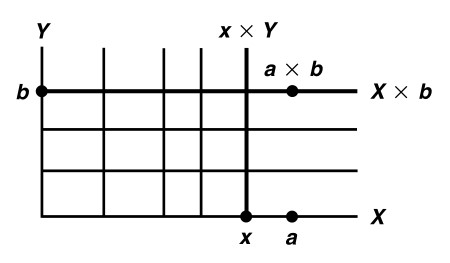
\includegraphics[ width = 0.6\linewidth ]{figures/Section 23/thm23-6.jpg}
            \caption{A visual of the slices and their intersections}
            \label{fig:23-6-1}
        \end{figure}

        Now form the union \( \bigcup_{ x \in X } T_{ x } \) of all of these 
        T-shaped spaces. We have that this union is connected because it is the
        union of a collection of connected spaces that have the point
        \( a \times b \) in common.
        Furthermore, we can see that this union equals \( X \times Y \), which
        tells us that \( X \times Y \) is connected.
    \end{proofBox}
\end{thmBox}

\begin{thmBox}{A Variant of Theorem 23.4}[thm:23.4-2]
    Let \( X \) be a topological space and let \( A \subset X \) be a subspace
    so \( \overline{ A } = X \).
    If \( A \) is connected, then \( X \) is connected.

    \baseRule

    \begin{proofBox}
        Let \( A \) be connected.
        Let us suppose that \( X \) is not connected.
        This means that there exists non-trivial clopen subsets of \( X \);
        let's suppose that \( B \) is a non-trivial clopen subset of \( X \).
        As a result, we have that \( X \setminus B \) is also a non-trivial 
        clopen subset of \( B \).
        Since \( A \) is connected, we see that it must be entirely contained
        in either \( B \) or \( X \setminus B \); WLOG, let's suppose that 
        \( A \) is entirely contained in \( B \).
        Since \( B \) is clopen (namely, closed) it must include all of its
        limit points, meaning that it must include the limit points of \( A \);
        in other words, since \( B \) is closed and contains \( A \), we have 
        that \( \overline{ A } \subset B \).
        However, we have that \( \overline{ A } = X \), which is impossible 
        since \( B \) is a non-trivial clopen subset of \( X \).
        Thus, we reach a contradiction and get that \( X \) must be connected.

        \baseRule

        Another approach to the proof is to look at \( B \cap A \).
        We see that \( B \cap A \) is clopen in \( A \) under the subspace 
        topology since \( B \) is clopen in \( X \).
        We need to show that \( B \cap A \) is non-trivial in \( A \) to 
        reach a contradiction.
        We start by showing that \( B \cap A \neq \emptyset \); since \( B \) 
        itself is non-trivial, we can pick a point \( p \in B \).
        \( B \) being clopen (namely, open) tells us that \( B \) is 
        an open neighborhood of \( p \).
        However, we have that \( p \in \mathrm{Cl} \ A = X \), which tells us 
        that \( B \) must intersect \( A \) non-trivially -- that is, we have
        \( B \cap A \neq \emptyset \).

        \baseSkip

        We now show that \( B \cap A \neq A \).
        To do so, let's pick any point \( q \in X \setminus B \).
        Since \( B \) is clopen (namely, closed), we see that 
        \( X \setminus B \) must then be open.
        Thus \( X \setminus B \) is an open neighborhood of \( q \).
        However, we also have that \( q \in \mathrm{Cl} \ A \), which tells
        us that \( ( X \setminus A ) \cap A \neq \emptyset \) -- that is, there
        is something in \( A \) that is not in \( B \).
        Thus, we have that \( B \cap A \neq A \).

        \baseSkip 

        Putting everything together gives us that \( B \cap A \) is a
        non-trivial clopen set of \( A \), which contradicts \( A \) being 
        connected.
    \end{proofBox}
\end{thmBox}